\documentclass[a4paper]{article}
\usepackage{times}
\usepackage[utf8]{inputenc}
\usepackage[T1]{fontenc}
\usepackage{selinput}
\usepackage{upquote}
\usepackage[margin=2cm, rmargin=4cm, tmargin=3cm]{geometry}
\usepackage{tcolorbox}
\tcbuselibrary{breakable}
\usepackage{xspace}
\usepackage{amsmath}
\usepackage{float}
\usepackage[french]{babel}
\usepackage{hyperref}
\usepackage{xurl}
\usepackage{fontawesome6}
\usepackage{enumitem}
\usepackage{marginnote}
\usepackage{ulem}
\usepackage[yyyymmdd,hhmmss]{datetime}
\usepackage{ulem}
\usepackage{environ}
\usepackage{graphicx}
%\usepackage[top=Bcm, bottom=Hcm, outer=Ccm, inner=Acm, heightrounded, marginparwidth=Ecm, marginparsep=Dcm]{geometry}
\usepackage{courier}



\newtcolorbox{Example}[1]{colback=white,left=20pt,colframe=slideblue,fonttitle=\bfseries,title=#1}
\newtcolorbox{Solutions}[1]{breakable,colback=white,left=20pt,colframe=green,fonttitle=\bfseries,title=#1}
\newtcolorbox{Conseils}[1]{colback=white,left=20pt,colframe=slideblue,fonttitle=\bfseries,title=#1}
\newtcolorbox{Warning}[1]{colback=white,left=20pt,colframe=warning,fonttitle=\bfseries,title=#1}
\newtcolorbox{Note}[1]{colback=white,left=20pt,colframe=grey,fonttitle=\bfseries,title=#1}
\newtcolorbox{Dessin}[1]{colback=white,left=20pt,colframe=grey,fonttitle=\bfseries,title=#1}

\setlength\parindent{0pt}

  %Exercice environment
  \newcounter{exercice}
  \newenvironment{Exercice}[1][]
  {
  \par
  \stepcounter{exercice}\textbf{Question \arabic{exercice}:} (\faClock \enskip \textit{#1})
  }
  {\bigskip}
  

% Title
\newcommand{\titre}{\begin{center}
  \section*{Algorithmes et Pensée Computationnelle}
\end{center}}
\newcommand{\cours}[1]
{\begin{center} 
  \textit{#1}\\
\end{center}
  }



% \newcommand{\exemple}[1]{\newline~\textbf{Exemple :} #1}
\newcommand{\todo}[1]{\textcolor{red}{#1}}
%\newcommand{\attention}[1]{\newline\faExclamationTriangle~\textbf{Attention :} #1}

% Documentation url (escape \# in the TP document)
\newcommand{\documentation}[1]{\faBookOpen~Documentation : \href{#1}{#1}}

% Clef API
\newcommand{\apikey}[1]{\faKey~Clé API : \lstinline{#1}}
\newcommand{\apiendpoint}[1]{\faGlobe~Url de base de l'API \href{#1}{#1}}

%Listing Python style
\usepackage{color}
\definecolor{slideblue}{RGB}{33,131,189}
\definecolor{green}{RGB}{0,190,100}
\definecolor{blue}{RGB}{121,142,213}
\definecolor{grey}{RGB}{120,120,120}
\definecolor{warning}{RGB}{235,186,1}

\usepackage{listings}
\lstdefinelanguage{texte}{
    keywordstyle=\color{black},
    numbers=none,
    frame=none,
    literate=
           {é}{{\'e}}1
           {è}{{\`e}}1
           {ê}{{\^e}}1
           {à}{{\`a}}1
           {â}{{\^a}}1
           {ù}{{\`u}}1
           {ü}{{\"u}}1
           {î}{{\^i}}1
           {ï}{{\"i}}1
           {ë}{{\"e}}1
           {Ç}{{\,C}}1
           {ç}{{\,c}}1
           {ô}{{\^o}}1,
    columns=fullflexible,keepspaces,
	breaklines=true,
	breakatwhitespace=true,
}
\lstset{
  language=Python,
	%basicstyle=\bfseries\footnotesize,
  basicstyle=\footnotesize\ttfamily\small,
	breaklines=true,
	breakatwhitespace=true,
	commentstyle=\color{grey},
	stringstyle=\color{slideblue},
  keywordstyle=\color{slideblue},
	morekeywords={with, as, True, False, Fraction, Float, join, index, None, main, argparse, self, sort, __eq__, __add__, __mul__ ,__ne__, __radd__, __del__, __ge__, __gt__, split, os, endswith, is_file, scandir, @classmethod, this},
	deletekeywords={id},
	showspaces=false,
	showstringspaces=false,
	columns=fullflexible,keepspaces,
	literate=
           {é}{{\'e}}1
           {è}{{\`e}}1
           {ê}{{\^e}}1
           {à}{{\`a}}1
           {â}{{\^a}}1
           {ù}{{\`u}}1
           {ü}{{\"u}}1
           {î}{{\^i}}1
           {ï}{{\"i}}1
           {ë}{{\"e}}1
           {Ç}{{\,C}}1
           {ç}{{\,c}}1
           {ô}{{\^o}}1,
    numbers=left,
}

\newtcbox{\mybox}{nobeforeafter,colframe=white,colback=slideblue,boxrule=0.5pt,arc=1.5pt, boxsep=0pt,left=2pt,right=2pt,top=2pt,bottom=2pt,tcbox raise base}
\newcommand{\projet}{\mybox{\textcolor{white}{\small projet}}\xspace}
\newcommand{\optionnel}{\mybox{\textcolor{white}{\small Optionnel}}\xspace}
\newcommand{\advanced}{\mybox{\textcolor{white}{\small Pour aller plus loin}}\xspace}
\newcommand{\auto}{\mybox{\textcolor{white}{\small Auto-évaluation}}\xspace}


\usepackage{environ}
\newif\ifShowSolution
\NewEnviron{solution}{
  \ifShowSolution
	\begin{Solutions}{\faTerminal \enskip Solution}
		\BODY
	\end{Solutions}
  \fi}

\usepackage{environ}
\newif\ifShowExample
\NewEnviron{exemple}{
  \ifShowExample
	\begin{Example}{\faTerminal \enskip Exemple}
		\BODY
	\end{Example}
  \fi}

\usepackage{environ}
 \newif\ifShowConseil
  \NewEnviron{conseil}{
    \ifShowConseil
    \begin{Conseils}{\faLightbulb \quad Conseil}
      \BODY
    \end{Conseils}

    \fi}

    \usepackage{environ}
  \newif\ifShowWarning
  \NewEnviron{attention}{
    \ifShowWarning
    \begin{Warning}{\faTriangleExclamation \quad Attention}
      \BODY
    \end{Warning}

    \fi}

  \newif\ifShowNote
  \NewEnviron{note}[1]{
    \ifShowNote
    \begin{Note}{\faEye \quad Comment added by #1 at \date - \currenttime}
      \BODY
    \end{Note}

    \fi}  

    \newif\ifShowDessin
    \NewEnviron{dessin}[1]{
      \ifShowDessin
      \begin{Dessin}{\faPen \quad Figure}
        \BODY
      \end{Dessin}
  
      \fi}  

%\newcommand{\Conseil}[1]{\ifShowIndice\ \newline\faLightbulb[regular]~#1\fi}

\usepackage{array}
\usepackage[T1]{fontenc}
\usepackage{tikz}
\usetikzlibrary{calc, backgrounds, arrows.meta, positioning}
\newcolumntype{C}[1]{>{\centering\let\newline\\\arraybackslash\hspace{0pt}}m{#1}}
\setlist[itemize]{label=\textbullet}

\begin{document}
% Change the following values to true to show the solutions or/and the hints
\ShowSolutionfalse
\ShowConseiltrue
\ShowExampletrue
\titre
    \cours{Algorithmes de recherche - Exercices de base}

Le but de cette séance est de se familiariser avec les algorithmes de recherche. Dans cette série d'exercices, nous manipulerons des listes et des collections en Python. Nous reviendrons sur la notion de récursivité et découvrirons les arbres binaires de recherche. Au terme de cette séance, vous serez en mesure d'effectuer des recherches de façon efficiente dans un ensemble de données.

\medskip
    
    Le code présenté dans les énoncés se trouve sur Moodle, dans le dossier \lstinline{code}.
    
    \section{Recherche séquentielle}
    \subsection{Définition}
    Une recherche \textbf{séquentielle} (ou \textbf{linéaire}) est une méthode permettant de trouver un élément dans un ensemble de données (liste, tableau, chaîne de caractères ou dictionnaire). Elle consiste à examiner les éléments un à un jusqu'à ce qu'une correspondance soit trouvée ou que tous les éléments aient été examinés. Dans un dictionnaire, ce parcours peut porter sur les clés, les valeurs ou les paires clé-valeur.\\
    
    Si l'élément recherché est trouvé, l'algorithme \textbf{renvoie l'index}, c'est-à-dire la position, de l'élément dans l'ensemble de données. \\
    
    Sa complexité est de $O(n)$, où $n$ est la longueur de la liste, car il faut parcourir toute la liste dans le pire des cas. \\
    
    \subsection{Exercices}
    
    \begin{Exercice}[20 minutes] [Python] Recherche séquentielle\\
    
    1. À partir des éléments ci-dessous, écrivez une fonction qui cherche un élément \texttt{e} dans la liste \texttt{liste}. \newline 
    
    La fonction renvoie l'index de l'élément correspondant de la liste si \texttt{e} est dans la liste et $-1$ si \texttt{e} n'est pas dans la liste.\\
    
    \textbf{Python:}
      \lstinputlisting{code/recherche_sequentielle.py}


\begin{conseil}
    Définissez votre fonction de recherche séquentielle en utilisant une boucle \lstinline{for} ou une boucle \lstinline{while}.
    
    Attention: la fonction renvoie l'index de la valeur et non la valeur elle-même. Pour cela:
    \begin{itemize}
        \item Avec une boucle \lstinline{for}, pensez à utiliser \lstinline{range(len(liste))}.
        \item Avec une boucle \lstinline{while}, utilisez une variable d'incrémentation \lstinline{i = i + 1}.
    \end{itemize}
    Affichez l'index retourné par la fonction de recherche. Si la valeur retournée est -1, affichez un autre message indiquant que l'élément n'était pas dans la liste.  
\end{conseil}
        
    \begin{solution}
    \textbf{Python:}
    \lstinputlisting[deletekeywords={index}]{solutions/recherche_sequentielle.py}
    L'implémentation retourne la première occurrence d'un élément, c'est pour ça que 2 est affiché et pas 5.
    \end{solution}

    2. Refaire la question en utilisant la fonction \lstinline{index} en Python.

    \begin{conseil}
        La fonction \lstinline|index| est appelée sur une liste \texttt{liste} afin de déterminer l'index d'un élément \texttt{e}: \lstinline{liste.index(e)}.
        \begin{itemize}
            \item Si \texttt{e} n'est pas dans la liste \texttt{liste}: la fonction lève une exception de type \lstinline{ValueError}. 
            \item Si \texttt{e} est dans la liste \texttt{liste}: la fonction retourne l'index de la première occurrence de \texttt{e}.
        \end{itemize}
    \end{conseil}

    \begin{solution}
        \textbf{Python:}
        % \lstinputlisting{solutions/recherche_sequentielle_index.py}
        \lstinputlisting[language=python, firstline = 1, firstnumber = 1, lastline = 14]{solutions/recherche_sequentielle_index.py}
    \end{solution}
    \begin{solution}
        \lstinputlisting[language=python, firstline = 17, firstnumber = 15]{solutions/recherche_sequentielle_index.py}
        La fonction \lstinline[language=python]|index| lève une exception si l'élément n'est pas présent, d'où l'utilisation de try/except.
    \end{solution}
    
    \end{Exercice}
    
    \begin{Exercice}[10 minutes] [Python] Recherche séquentielle \\
    
    Soit une liste d'entiers \textbf{non triée} \texttt{liste} ainsi qu'un entier \texttt{e}. Écrivez un programme qui retourne l'élément de la liste \lstinline{liste} dont la valeur est la plus proche de \texttt{e} en utilisant une recherche séquentielle.\\
    \begin{exemple}
        \lstinputlisting[language=python, firstline=18, firstnumber=1, lastline=24]{solutions/plus_proche_sequentielle.py}
    \end{exemple}
    Au cas où deux éléments se trouveraient à équidistance de \lstinline{e}, renvoyez l'élément le plus petit.\\
    
    \textbf{Python :}
        \lstinputlisting{code/plus_proche_sequentielle.py}
        \begin{conseil}
        Complétez la fonction \texttt{plus\_proche\_sequentielle} puis exécutez le code. \\

        Pour comparer les écarts, utilisez les valeurs absolues, car la différence la plus petite peut être positive ou négative. En Python, la fonction \lstinline{abs()} retourne la valeur absolue d'un nombre. Par exemple: \lstinline{abs(3 - 10)} retourne 7.\\

        Étant donné que la liste n'est \textbf{pas triée}, l'algorithme doit nécessairement la parcourir entièrement. \\

        L'algorithme doit calculer la différence entre \texttt{e} et chaque élément de la liste \texttt{liste}, tout en conservant en mémoire la plus petite différence rencontrée. À la fin, il retourne l'élément de la liste correspondant à la plus petite différence.
        \end{conseil}
        
        \begin{solution}
        \textbf{Python :}
            \lstinputlisting{solutions/plus_proche_sequentielle.py}
        \end{solution}
        
    \end{Exercice}
    
    \section{Recherche binaire — Binary search}
    
    \subsection{Définition}
    
    Le but de la recherche binaire est de trouver l'élément recherché de façon optimale. Pour cela, il est nécessaire d'utiliser \textbf{une liste d'éléments triés}.\\
    
    La complexité de l'algorithme de recherche binaire est \lstinline{O(log n)}. Cependant, il ne faut pas oublier le coût lié à l'obtention d'une liste triée à partir d'une liste non triée.\\
    
    L'algorithme de recherche binaire divise l'intervalle de recherche par deux à chaque itération jusqu'à ce qu'il trouve l'élément \lstinline{key} ou que l'intervalle soit vide.\\
    
    Ainsi, si \lstinline{key} est plus petit que l'élément du milieu, l'algorithme va choisir la moitié de gauche comme intervalle de recherche et ainsi de suite. Si \lstinline{key} est plus grand que l'élément du milieu la recherche va se faire dans la moitié droite de l'intervalle.\\
    
    La recherche binaire se base sur les comparaisons d'ordre, alors que la recherche séquentielle se base sur les comparaisons d'égalité pour trouver l'élément recherché.\\
    
    \subsection{La récursivité}
    
    Une fonction récursive est une fonction qui s'appelle elle-même pendant son exécution. Vous trouverez ci-dessous un exemple de fonction récursive utilisée pour effectuer un calcul factoriel.\\\\
    (Rappel : 4! = 4 x 3 x 2 x 1 = 24)\\
    
    \lstinputlisting{code/factorial.py}
    
    Les fonctions récursives sont courantes en informatique car elles permettent aux programmeurs d'écrire des programmes efficaces en utilisant une quantité minimale de code. Leur principal inconvénient est le fait qu'elles peuvent provoquer des exécutions infinies et d'autres résultats inattendus si elles ne sont pas écrites correctement. Si la fonction n'inclut pas les cas permettant d'arrêter la récursivité, celle-ci se répétera à l'infini, provoquant le plantage du programme ou, pire encore, l'arrêt de tout le système informatique.\\
       
    \subsection{Exercices}

    
    \begin{Exercice}[20 minutes] [Python] Algorithme de recherche binaire — Binary search\\
    
    À partir de la liste d'éléments \textbf{triés} ci-dessous, écrivez premièrement \textbf{une fonction récursive} puis \textbf{une fonction itérative} qui cherche \texttt{key} dans la liste. La fonction renvoie \textbf{l'index} de l'élément correspondant de la liste si \texttt{key} est dans la liste et \lstinline{-1} dans le cas contraire.\\

    Testez votre implémentation avec la liste \texttt{liste=[1,3,4,5,7,8,9,15]} dans laquelle vous cherchez \texttt{key=7}. Combien d'appels à la fonction de recherche binaire récursive sont effectués?
    
    \subsubsection*{Question 3.1 - Version récursive}
    \lstinputlisting{code/recherche_binaire_recursive.py}
    
    \subsubsection*{Question 3.2 - Version itérative}
    \lstinputlisting{code/recherche_binaire_iterative.py}
    
    
        \begin{conseil}
            Complétez la fonction récursive \lstinline{recherche_binaire_recursive} et la fonction itérative \lstinline{recherche_binaire}.\\\\
            Détails sur les arguments de la fonction \lstinline{recherche_binaire_recursive}:
            \begin{itemize}
            \item \lstinline{key}: La valeur recherchée.
            \item \lstinline{array}: La liste dans laquelle nous effectuons la recherche.
            \item \lstinline{low}: L'indice de départ de la partie de la liste à fouiller (0 au départ).
            \item \lstinline{high}: Le dernier indice de la partie de la liste à fouiller (\lstinline{len(array) - 1} au départ).
            \end{itemize}
            Ainsi, à chaque itération, vos fonctions vont modifier les valeurs de base données en argument pour resserrer l'intervalle jusqu'à trouver la valeur recherchée.\\        
            
            Pour la version itérative, il est conseillé d'utiliser une boucle \lstinline{while}. Pour la fonction \lstinline{recherche_binaire}, les seuls arguments sont la liste \texttt{liste} et l'élément à chercher \lstinline{key}. 
        \end{conseil}

        \begin{conseil}
            Pour définir le milieu d'une liste qui contient un nombre pair ou impair d'éléments, divisez l'ensemble en 2 et utilisez la fonction \lstinline{int()} pour convertir le résultat en entier. 
            \lstinputlisting{solutions/midpoint.py}
        \end{conseil}
    
        \begin{solution}
            \subsubsection*{3.1 - Version récursive}
            \lstinputlisting{solutions/recherche_binaire_recursive.py}
        \end{solution}
        \begin{solution}
            \subsubsection*{3.2 - Version itérative}
            \lstinputlisting{solutions/recherche_binaire_iterative.py}
        \end{solution}
        \begin{solution}
        \begin{minipage}{\linewidth}
        \textbf{Appels de la recherche binaire récursive}

        \begin{center}
        \begin{tikzpicture}[
            font=\footnotesize,
            cell/.style={draw, minimum width=0.75cm, minimum height=0.6cm,
                         inner sep=0pt, font=\small},
            idx/.style={font=\scriptsize, text=gray, inner sep=1pt},
            marker/.style={font=\scriptsize\ttfamily, text=slideblue!80!black,
                           inner sep=1pt},
            callnum/.style={circle, fill=slideblue, text=white, inner sep=1.5pt,
                         font=\scriptsize\bfseries},
            callarrow/.style={-Stealth, thick, slideblue},
            retarrow/.style={-Stealth, thick, dashed, green!50!black},
            cmp/.style={anchor=west, align=left, text width=3cm}
        ]
        % Une ligne par appel : numéro / low / high / mid / ordonnée
        \foreach \r/\lo/\hi/\mi/\y in {1/0/7/3/0, 2/4/7/5/-2.4, 3/4/4/4/-4.8}{
            \foreach \v [count=\i from 0] in {1,3,4,5,7,8,9,15}{
                % Hors de [low, high] : grisé ; dans l'intervalle : bleu
                \def\fillc{slideblue!8}\def\drawc{slideblue!70}\def\textc{black}
                \def\lw{0.4pt}
                \ifnum\i<\lo \def\fillc{gray!8}\def\drawc{gray!40}\def\textc{gray!60}\fi
                \ifnum\i>\hi \def\fillc{gray!8}\def\drawc{gray!40}\def\textc{gray!60}\fi
                % Élément du milieu : orange (vert s'il est trouvé)
                \ifnum\i=\mi
                    \def\fillc{orange!30}\def\drawc{orange!80!black}\def\lw{1.2pt}
                    \ifnum\r=3 \def\fillc{green!30}\def\drawc{green!50!black}\fi
                \fi
                \node[cell, fill=\fillc, draw=\drawc, text=\textc,
                      line width=\lw] (r\r-\i) at (\i*0.75, \y) {\v};
                \node[idx, above=0pt of r\r-\i] {\i};
            }
            \node[callnum] (s\r) at (-0.9, \y) {\r};
        }

        % Appels effectués
        \node[anchor=south west] at ($(r1-0.north west)+(0,0.3)$)
            {\texttt{recherche\_binaire\_recursive(7, liste, 0, 7)}};
        \node[anchor=south west] at ($(r2-0.north west)+(0,0.3)$)
            {\texttt{recherche\_binaire\_recursive(7, array, 4, 7)}};
        \node[anchor=south west] at ($(r3-0.north west)+(0,0.3)$)
            {\texttt{recherche\_binaire\_recursive(7, array, 4, 4)}};

        % Positions de low, mid et high
        \node[marker, below=1pt of r1-0] {low};
        \node[marker, below=1pt of r1-3] {mid};
        \node[marker, below=1pt of r1-7] {high};
        \node[marker, below=1pt of r2-4] {low};
        \node[marker, below=1pt of r2-5] {mid};
        \node[marker, below=1pt of r2-7] {high};
        \node[marker, below=1pt of r3-4] {low = mid = high};

        % Comparaisons
        \node[cmp] (c1) at ($(r1-7.east)+(0.4,0)$)
            {$\texttt{array[3]} = 5 < 7$\\ $\Rightarrow$ moitié droite};
        \node[cmp] (c2) at ($(r2-7.east)+(0.4,0)$)
            {$\texttt{array[5]} = 8 > 7$\\ $\Rightarrow$ moitié gauche};
        \node[cmp] (c3) at ($(r3-7.east)+(0.4,0)$)
            {$\texttt{array[4]} = 7 = \texttt{key}$\\ $\Rightarrow$ \texttt{return 4}};

        % Appels récursifs (descente) et valeurs de retour (remontée)
        \draw[callarrow] (s1) -- (s2);
        \draw[callarrow] (s2) -- (s3);
        \draw[retarrow] ([yshift=-2pt]c3.east) to[bend right=50]
            node[right] {\texttt{4}} ([yshift=-2pt]c2.east);
        \draw[retarrow] ([yshift=2pt]c2.east) to[bend right=50]
            node[right] {\texttt{4}} ([yshift=2pt]c1.east);
        \end{tikzpicture}
        \end{center}

        Chaque ligne correspond à un appel : les cases bleues forment
        l'intervalle \texttt{[low, high]} encore à fouiller, la case orange
        est l'élément du milieu comparé à \texttt{key} et la case verte est
        l'élément trouvé. Les flèches bleues indiquent les appels récursifs
        et les flèches vertes en pointillés le retour de l'indice \texttt{4}.

        \medskip

        La fonction est appelée \textbf{trois fois au total}, soit l'appel
        initial et \textbf{deux appels récursifs}. Chaque appel renvoie
        l'indice \texttt{4} à son appelant.
        \end{minipage}
        \end{solution}
    
    \end{Exercice}
    
    \section{Arbre binaire de recherche — Binary search tree}
    \subsection{Définition}
    
    Un arbre binaire de recherche est une structure de données au même titre que les listes, tuples, dictionnaires, etc. La particularité de ces arbres est qu'au lieu d'ordonner les éléments les uns à la suite des autres, les arbres binaires de recherche enregistrent les valeurs de manière relationnelle.\\
    
    En effet, l'arbre est divisé en branches qui peuvent elles-mêmes contenir deux branches (enfants) et ainsi de suite. Lorsqu'une branche n'a pas de branches subséquentes (enfants), on parle de feuille.\\
    
    Les branches peuvent donc contenir de 0 à 2 autres branches. On parle alors de branche de gauche et de celle de droite. La branche de gauche est forcément plus petite que la branche parente et celle de droite est forcément plus grande.\\
    
    De cette façon, on garantit que l'arbre est toujours ordonné même en rajoutant ou en retirant des éléments\\
    
    \begin{figure}[H]
        \centering
        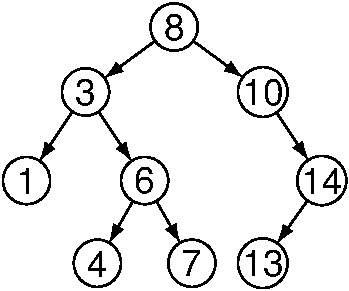
\includegraphics[width=0.32\textwidth]{img/binary-search-tree.pdf}
        \caption{Exemple d'arbre binaire de recherche}
    \end{figure}
    
    \subsection{Exercices}

    \begin{Exercice}[10 minutes] Propriété des arbres binaires de recherche\\

    Supposons que nous ayons des nombres entre 1 et 1000 dans un arbre binaire de recherche, et que nous voulions rechercher le nombre 363. Lesquelles des séquences suivantes ne pourraient pas être une séquence des nœuds examinés avant de trouver 363 ?

    \begin{enumerate}
        \item 2, 252, 401, 398, 330, 344, 397, 363.
        \item 924, 220, 911, 244, 898, 258, 362, 363.
        \item 925, 202, 911, 240, 912, 245, 363.
        \item 2, 399, 387, 219, 266, 382, 381, 278, 363.
        \item 935, 278, 347, 621, 299, 392, 358, 363. 
    \end{enumerate}

    \begin{conseil}
        Rappelez-vous la propriété suivante des arbres binaires de recherche:
        \begin{center}
   \begin{tikzpicture}[
    node distance=1.5cm,
    every node/.style={circle, draw, fill=gray!30, minimum size=0.8cm},
    every path/.style={thick}
]

% 1. Define Nodes first (so we can reference their positions)
\node (z) at (0,0) {$z$};
\node (l) at (-1.7,-1.5) {$l$};
\node (r) at (1.7,-1.5) {$r$};

% 2. Edges
\draw (z) -- (l);
\draw (z) -- (r);

% Dashed lines for children
\draw[dashed] (l) -- ++(-0.95,-0.95);
\draw[dashed] (l) -- ++(0.95,-0.95);
\draw[dashed] (r) -- ++(-0.95,-0.95);
\draw[dashed] (r) -- ++(0.95,-0.95);
\draw[dashed] (z) -- ++(0,0.95);

% 3. Background Rectangles
% We use 'on background layer' to push these behind the nodes defined above
\begin{scope}[on background layer]
    \fill[red!10, opacity=0.6, rounded corners] 
        ($(z.north east) + (-0.4,-1.2)$) rectangle ($(l.south west) + (-1.4,-1.9)$);
        
    \fill[blue!10, opacity=0.7, rounded corners] 
        ($(z.north east) + (3.1,-1.2)$) rectangle ($(l.south west) + (2.1,-1.9)$);
\end{scope}

% 4. Text Descriptors
\node[
  rectangle,
  draw=none,
  fill=none,
  align=left,
  text width=4cm
] at (-0.95, -3) {Tous les nœuds \\ (y compris $l$) $<$ $z$};

\node[
  rectangle,
  draw=none,
  fill=none,
  align=left,
  text width=2.8cm
] at (1.9, -3) {Tous les nœuds \\ (y compris $r$) $>$ $z$};

\end{tikzpicture}
\end{center}
Tous les nœuds dans le sous-arbre à gauche ont une valeur inférieure à la valeur du nœud $z$ et tous les nœuds dans le sous-arbre à droite ont une valeur supérieure à la valeur du nœud $z$.
    \end{conseil}
    \begin{solution}
            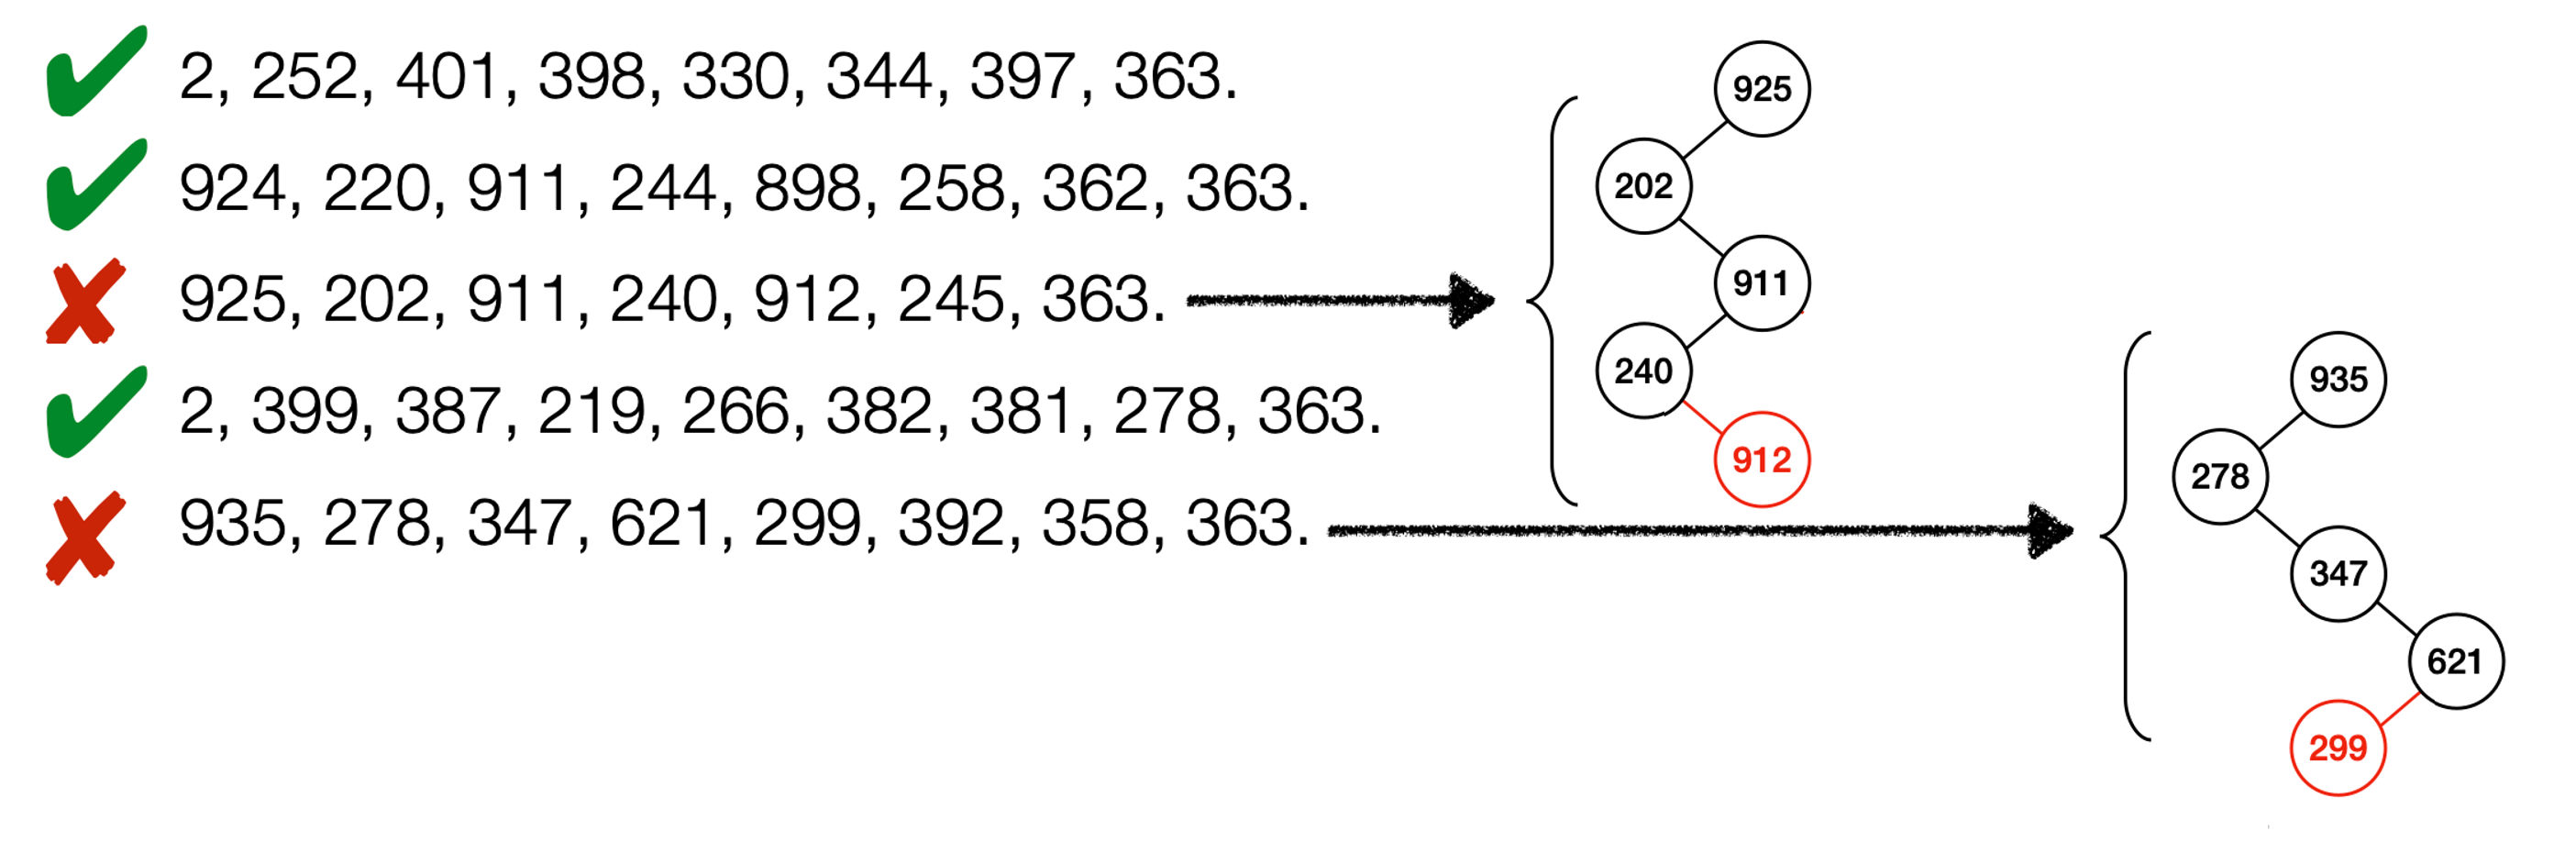
\includegraphics[width=1\textwidth]{img/question4.png}
        \begin{itemize}
            \item Le troisième choix est faux car 912 se trouve dans le sous-arbre à gauche de 911 ce qui contredit la propriété des arbres binaires de recherche.
            \item Le cinquième choix est faux car 299 se trouve dans le sous-arbre à droite de 347 ce qui contredit la propriété des arbres binaires de recherche.
        \end{itemize}  
    \end{solution}

        
    \end{Exercice}
    
    \begin{Exercice}[20 minutes] [Python] Recherche dans un arbre\\
        
        Dans l'exercice suivant, nous vous donnons un arbre binaire de recherche avec les mêmes valeurs que le schéma précédent et dont la racine est la variable \lstinline{root}.\\
    
        Écrivez une fonction qui retourne \lstinline{True} si la valeur \lstinline{e} se trouve dans l'arbre et \lstinline{False} dans le cas contraire. Pour un nœud \lstinline{node}, utilisez l'attribut \lstinline{node.value} pour accéder à sa valeur et les attributs \lstinline{node.left} et \lstinline{node.right} pour accéder à ses sous-arbres gauche et droit.\\\\
        Complétez la fonction \lstinline{recherche_arbre}.\\
        \begin{lstlisting}[language=Python]
def recherche_arbre(node, e):
    # Complétez ici
    
    
#Attention à inclure les lignes de code additionnelles présentes dans le fichier "arbre_recherche_binaire.py" sur Moodle
        \end{lstlisting}
    
        \begin{conseil}
        Indice: Utilisez une fonction récursive.\\
        
        Pour cette question, vous devez télécharger le fichier \textbf{arbre\_recherche\_binaire.py} sur Moodle et copier tout son contenu dans votre fichier Python. Celui-ci contient les classes permettant de définir les arbres selon le concept vu en cours. \\
        
        Il contient également un code de ``vérification''. Celui-ci va automatiquement tester votre fonction avec différents paramètres et vérifier si les résultats obtenus correspondent aux résultats attendus.
        \end{conseil}
    
        \begin{solution}
            \lstinputlisting{solutions/recherche_arbre.py}
        \end{solution}
    
    \end{Exercice}
    
    \end{document}
